\documentclass[14pt,aspectratio=169]{beamer}

% Assets
\usepackage[czech]{babel}				% Jazyk
\usepackage[a-2u]{pdfx}					% Kopírování z pdfka
\usepackage{tikz}						% Schémata automatů
\usepackage{csquotes}					% české uvozovky
\usepackage{enumerate}					% enumerate environment
\usepackage{indentfirst}
\usepackage{mathtools}
\usepackage{pifont}
\usepackage{xcolor}
\usepackage{enumitem,xcolor}
\usepackage{amsmath}
\usepackage[utf8]{inputenc}

\usepackage{listings}                   % Úryvky z kódu (C#)
\lstset{language=[Sharp]C, frame=lr}
% Beamer theme
\usetheme{Boadilla}
\setbeamertemplate{frame numbering}[fraction]
\usecolortheme[named=black]{structure}
\setbeamertemplate{navigation symbols}{}
\setbeamerfont{title}{series=\bfseries,parent=structure}
\setbeamerfont{frametitle}{series=\bfseries,parent=structure}
\usefonttheme[onlymath]{serif}
\urlstyle{same}

% Dark theme
\setbeamercolor{frametitle}{fg=white}
\setbeamercolor{title}{fg=white}
\setbeamercolor{background canvas}{bg=black}
\setbeamercolor{normal text}{fg=white}

\defbeamertemplate*{title page}{customized}[1][]
{ 
  \usebeamerfont*{title}\inserttitle\par
  \bigskip
  \usebeamerfont*{subtitle}\textit{\insertsubtitle}\par
  \bigskip \bigskip \bigskip \bigskip 
  \usebeamerfont{author}\insertauthor\par
  \usebeamerfont{institute}Kabinet \office\\\url{weber3@spsejecna.cz}\bigskip
}
% Enumerate
%\setlist[enumerate]{topsep=0pt,itemsep=-1ex,partopsep=1ex,parsep=1ex,label=(\arabic*)}

\MakeOuterQuote{"}

% Colors
\definecolor{lightblue}{HTML}{009AD4}
\definecolor{darkgreen}{HTML}{0D7103}
\definecolor{lightgreen}{HTML}{68FF00}
\definecolor{darkred}{HTML}{AF0B0B}
\definecolor{lightred}{HTML}{FF5100}
\definecolor{orange}{HTML}{FFE000}
\definecolor{codeblue}{HTML}{FF0055}
\definecolor{codegreen}{rgb}{0,0.6,0}
\definecolor{codegray}{rgb}{0.5,0.5,0.5}
\definecolor{codebeige}{HTML}{D4A000}
\definecolor{backcolour}{rgb}{0.95,0.95,0.92}

\newcommand{\markred}[1]{\textcolor{lightred}{#1}}
\newcommand{\markgreen}[1]{\textcolor{lightgreen}{#1}}
\newcommand{\markorange}[1]{\textcolor{orange}{#1}}
\newcommand{\markblue}[1]{\textcolor{lightblue}{#1}}

% Inline images
\newcommand{\inlineimgscale}{1.1}

% X and check mark
\newcommand{\cmark}{\markgreen{\ding{51}}}
\newcommand{\xmark}{\markred{\ding{55}}}

% Redefinions
\renewcommand{\implies}{\Rightarrow}
\renewcommand{\impliedby}{\Leftarrow}

% Math
\newcommand{\R}{\mathbb{R}}
\newcommand{\C}{\mathbb{C}}
\newcommand{\N}{\mathbb{N}}
\newcommand{\Z}{\mathbb{Z}}
\newcommand{\Q}{\mathbb{Q}}

% Code
\lstdefinestyle{clang}{
    basicstyle=\small\ttfamily\color{white},
    language=C,
    keywordstyle=\color{codeblue},
    commentstyle=\color{codegreen},
    numberstyle=\tiny\color{codegray},
    stringstyle=\color{codebeige},
    breakatwhitespace=false,
    breaklines=true,
    captionpos=b,
    keepspaces=true,
    numbersep=5pt,
    showspaces=false,
    showstringspaces=false,
    showtabs=false,
    morekeywords={void,int,double,float,unsigned,if,else,\#include}
    tabsize=0.5
}
\lstset{escapeinside={(*}{*)},style=clang}

\newcommand{\hlcode}[1]{\colorbox{red}{#1}}

% Title page
\title{Informační a komunikační technologie}
\subtitle{Práce s polem}
\author{David Weber}
\def\office{K13}
\def\email{weber3@spsejecna.cz}

\begin{document}

    % Itemize
    \setlist[itemize]{label=\textcolor{white}{\textbullet}}

    % Slides
    \begin{frame}
        \titlepage
    \end{frame}

    \begin{frame}[t,fragile]{Jak jsme zatím pracovali\dots}
        \begin{itemize}
            \item Zatím jsme pracovali se samostatnými proměnnými
            \item Např. načtení rozměrů obdélníku
            \begin{lstlisting}
float width, height;
scanf("%d %d", &width, &height);
            \end{lstlisting}
            \item \markgreen{Funguje pro pevný počet hodnot.} \emoji{slightly-smiling-face}
            \item \markred{Nefunguje pro proměnný počet hodnot.} \emoji{worried-face}
        \end{itemize}
    \end{frame}

    \begin{frame}[t]{Co použít?}
        \begin{itemize}
            \item Můžeme se dostat do situace, kde počet hodnot, které potřebujeme uchovat, závisí buď přímo na uživateli, nebo na jiných okolnostech
            \item $\implies$ pro uchování většího množství hodnot \textbf{stejného datového typu} používáme tzv. \textbf{pole} (anglicky \emph{array}).
            \item Lze si představit jako "řadu přihrádek"
            \begin{figure}
                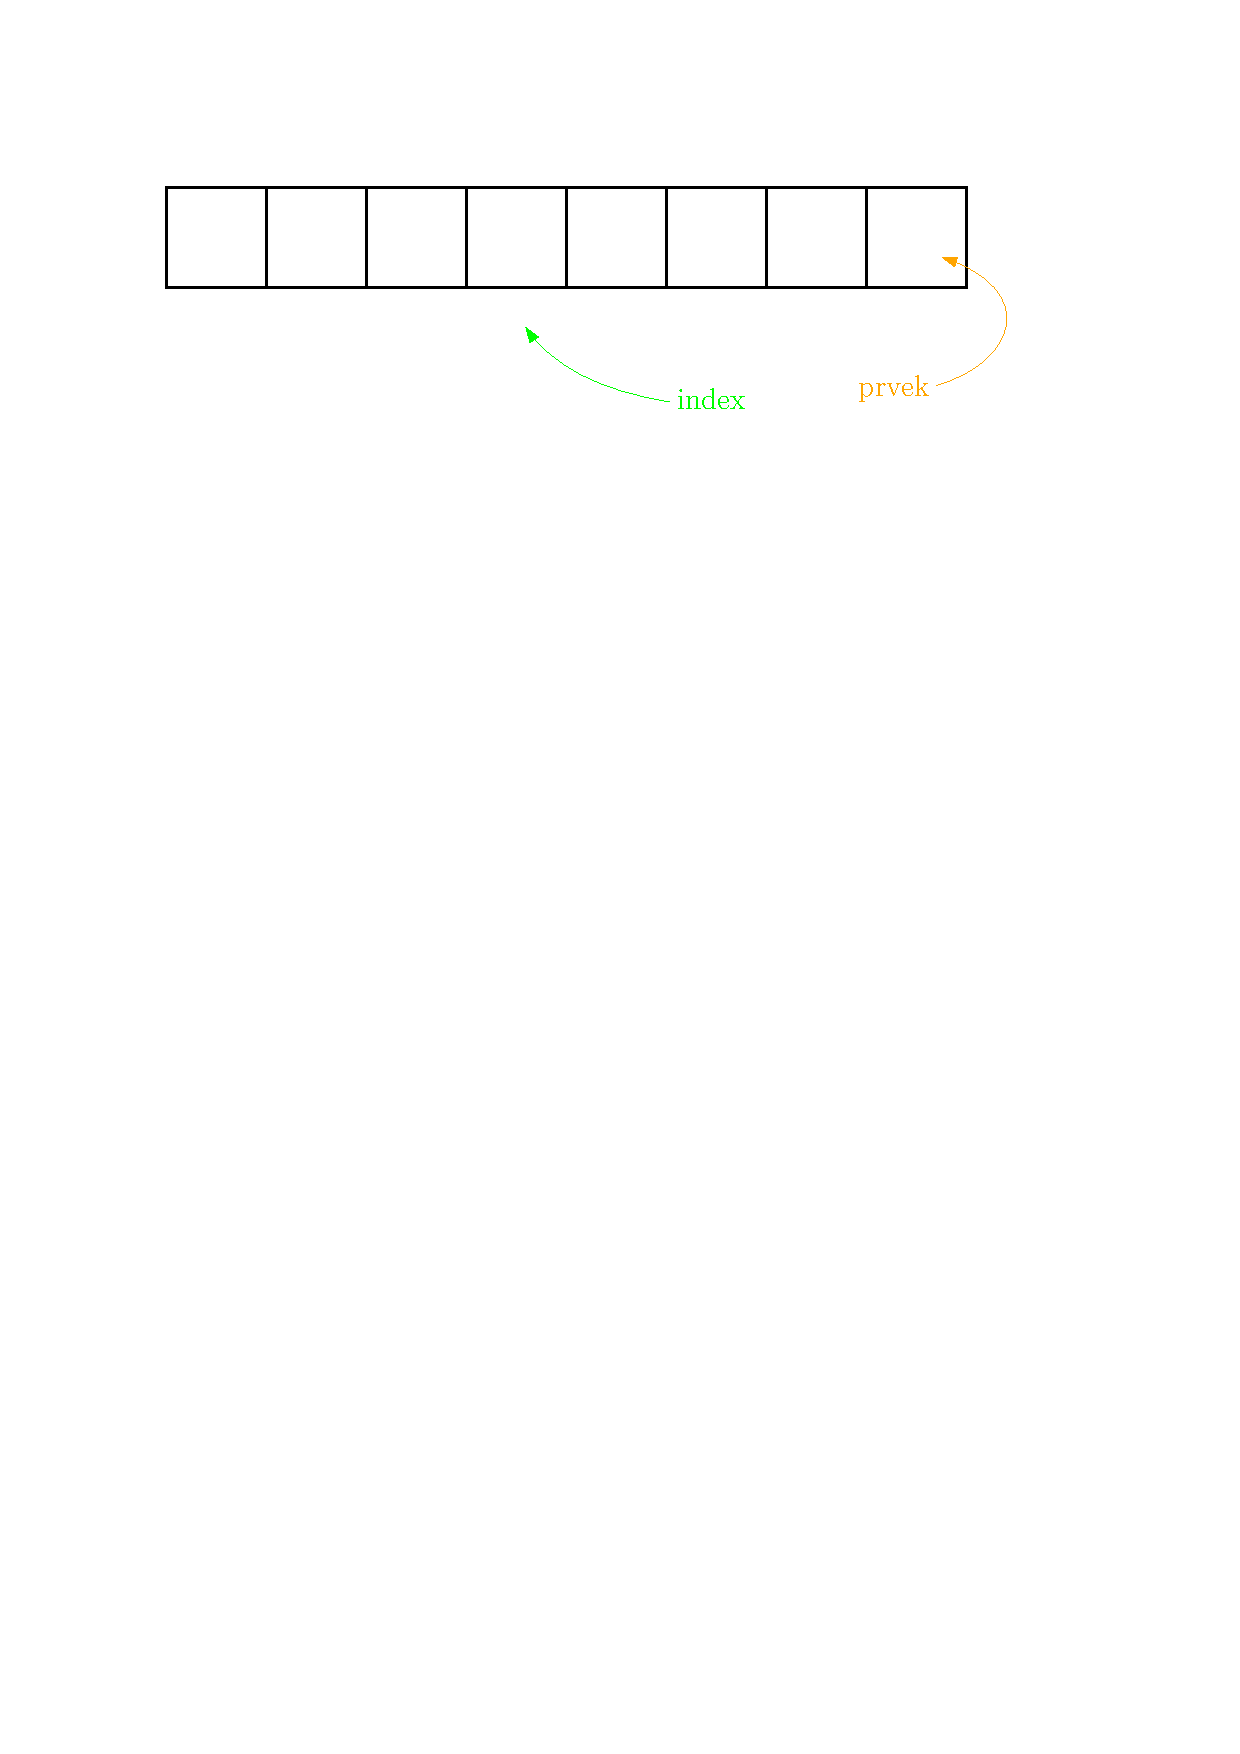
\includegraphics[scale=.8]{images/array1.pdf}
            \end{figure}
        \end{itemize}
    \end{frame}

    \begin{frame}[t,fragile]{Vlastnosti pole I}
        \begin{itemize}
            \item Každý prvek má v poli svoji pozici (index), které se číslují \textbf{od nuly}.
            \item Pro obecný počet prvků $n$ máme tak indexy $0,\,1,\,2,\,\dots,\,n-1$.
            \item Pole deklarujeme pomocí \textbf{datového typu prvků} a jeho \textbf{velikosti (tj. počtu prvků)}. Např.
            \begin{lstlisting}
int array[10];
            \end{lstlisting}
            \item Případně lze rovnou deklarovat pole i s uchovanými hodnotami:
            \begin{lstlisting}
int array[] = { -1, 0, 2023, 40 };
            \end{lstlisting}
            \item V takovém případě nemusíme uvádět velikost.
        \end{itemize}
    \end{frame}

    \begin{frame}[t,fragile]{Vlastnosti pole II}
        \begin{itemize}
            \item K prvkům přistupujeme pomocí jejich \textbf{indexu}, který uvádíme do hranatých závorek.
            \begin{lstlisting}
int array[10];
array[0] = 1;
array[3] = -10;
            \end{lstlisting}
            \item Podobně můžeme např. vypsat daný prvek v poli či načíst hodnotu na vstupu:
            \begin{lstlisting}
scanf("%d", &array[7]);
printf("%d", array[7]);
            \end{lstlisting}
        \end{itemize}
    \end{frame}

    \begin{frame}[t,fragile]{Příklad (1/2)}
        Výpis všech zadaných prvků:
        \begin{lstlisting}
// Load array length
int count;
scanf("%d", &count);

int numbers[count];
        \end{lstlisting}
    \end{frame}

    \begin{frame}[t,fragile]{Příklad (2/2)}
        \begin{lstlisting}
// Fetch numbers into array
int i;
for (i = 0; i < count; i++){
    scanf("%d", &numbers[i]);
}

// Print array
for (i = 0; i < count; i++){
    printf("%d ", numbers[i]);
}

return 0;
        \end{lstlisting}
    \end{frame}

    \begin{frame}[t,fragile]{Vlastnosti pole III}
        \begin{itemize}
            \item Co když zasáhnu indexem mimo pole?
            \begin{lstlisting}
int arr[5];
arr[7] = ...;
            \end{lstlisting}
            \item \markred{Jazyk C toto neošetřuje $\implies$ zasáhneme mimo blok paměti pole!}
            \begin{figure}
                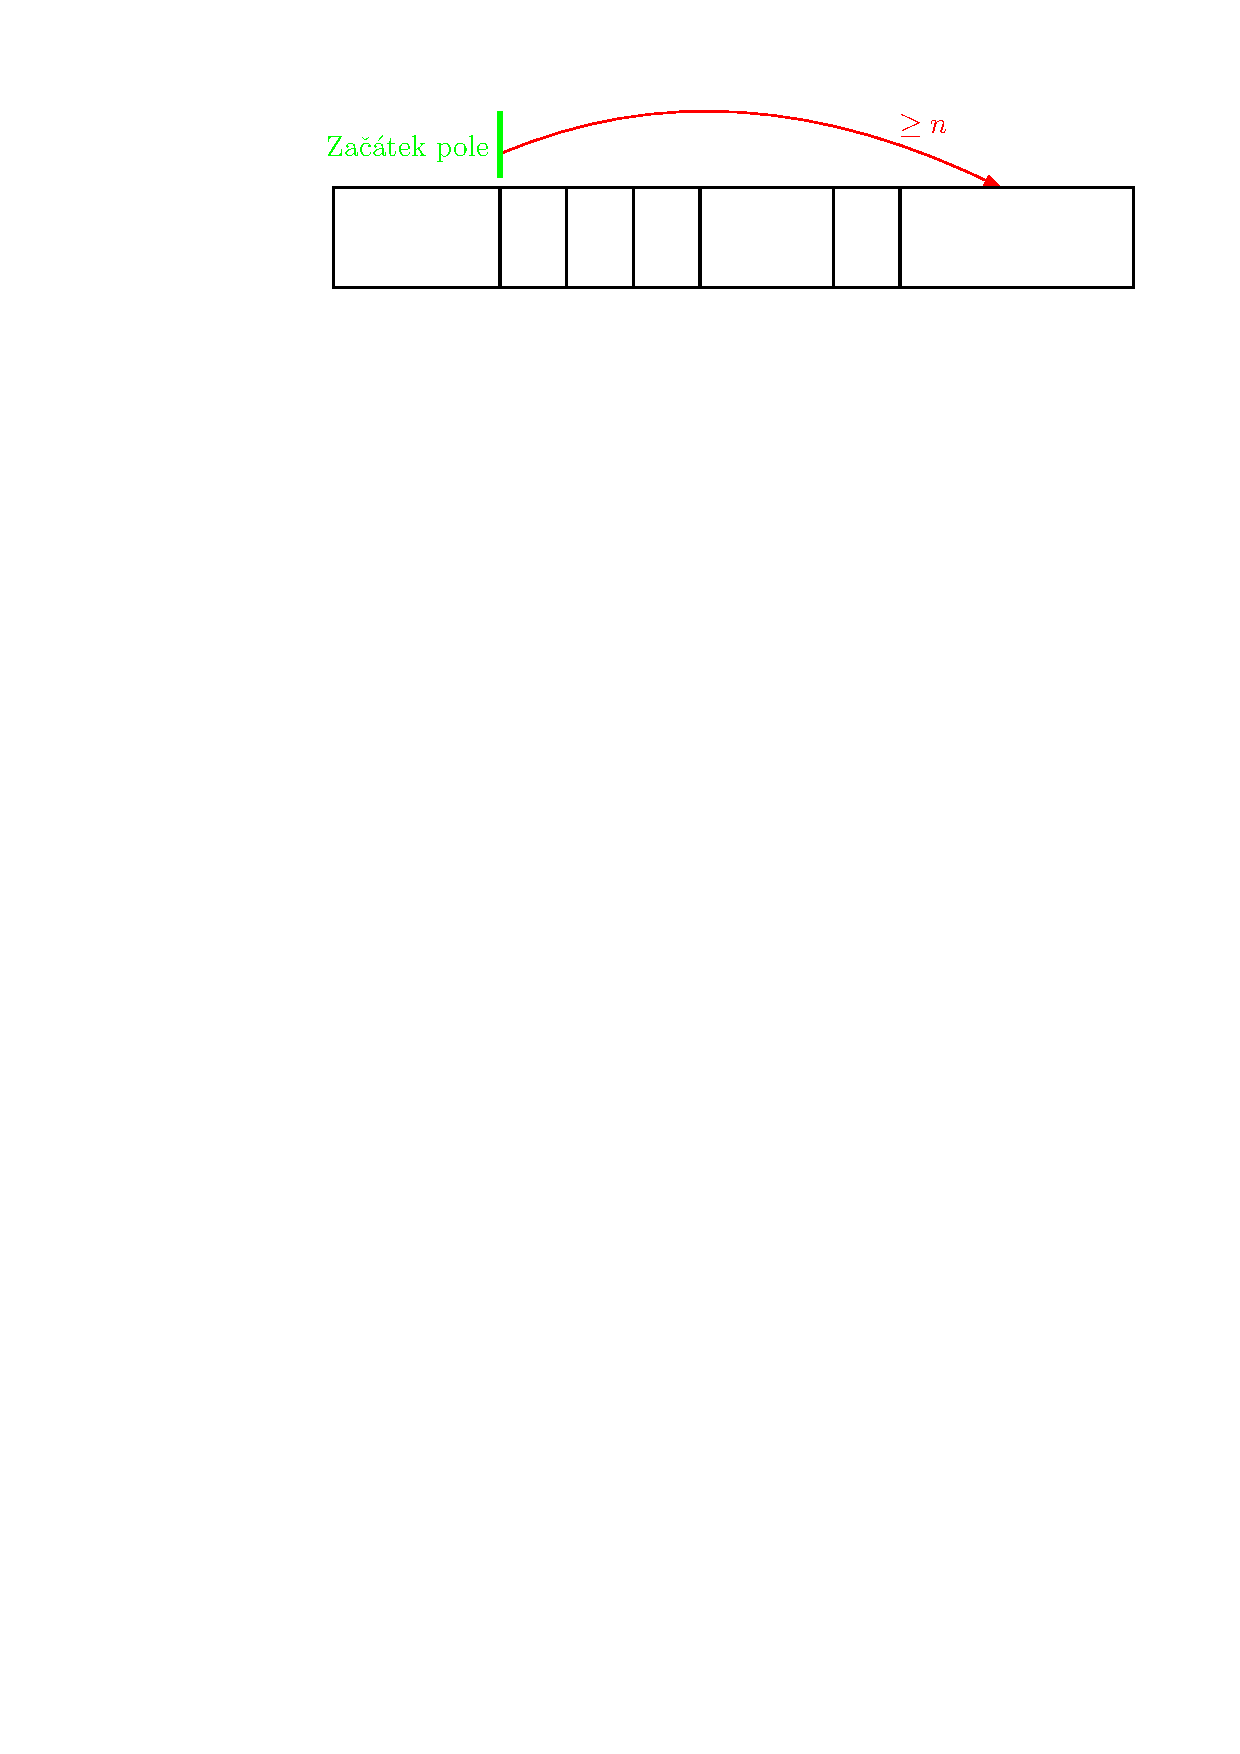
\includegraphics[scale=.8]{images/array_memory.pdf}
            \end{figure}
            \item Může tak dojít k přepisu jiné proměnné
        \end{itemize}
    \end{frame}

    \begin{frame}{Otázky?}
        \begin{figure}
            \centering
            
\includegraphics[scale=.4]{images/discussion_inverted.png}
        \end{figure}
    \end{frame}

\end{document}